%\documentclass[11pt,a4paper]{article}
%\documentclass[class=book,twocolumn]
\documentclass[./exercises.tex]{subfiles}

\begin{document}

%\begin{multicols}{2}
\bigskip
\noindent\textbf{5.1-94}\hfill\break
\noindent En ideal gas genomlöper följande kretspro-\\
cess medudurs
\begin{table}[ht]
\noindent\begin{tabular}{ l l  } 
1 $\rightarrow$ 2 & Isentropisk kompression\\
2 $\rightarrow$ 3 & Tryckökning vid konstant volym  \\ 
3 $\rightarrow$ 4 & Polytropisk expansion $(n=1.2)$.\\
4 $\rightarrow$ 1 & Tryckminskning vid konstant volym.\\                
\end{tabular}
\end{table}

Rita processen i $p$\,-$V$- och $T$-$s$-diagrammen.
Bestäm termiska verkningsgraden då $T_1=300$K. $T_3=700$K, $T_4=500K$ och $\kappa=1.4$.
\bigskip

\begin{figure}[h]
\centering
%%%%%%%%%%%%%%%p-V-diagram
\subfigure[$p\, \mhyphen V$ diagram] 
{
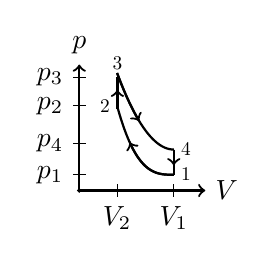
\begin{tikzpicture}[ scale=.4,baseline={(0,0)}]
%\draw (0,0) grid (4,4);
% x-axis
\draw [thick,->] (0,0) -- (4,0) node[right]{$V$};
% y-axis
\draw [thick,->] (0,0) -- (0,4) node[above] {$p$};
% origin point
\draw [color=black,fill=black] (0,0) circle (0.05);

%Isentropisk kompression från x1=3.5, y1=0.5 till x2=0.6, y2=2
%y= y0+(y1-y2)*abs((x-x2)/(x2-x1))^n
%\draw[ thick,->,domain=3.5:0.6, smooth, variable=\x, black] plot ({\x}, {0.716*abs(\x-3.5)^1.4 -0.5});
%\draw[ thick,domain=3.5:0.6, smooth, variable=\x, black] plot ({\x}, {(0.5+(2-0.5)*(abs((\x-0.6)/(0.6-3.5)))^2}) node[scale=0.7, left]{2};
\draw[ thick,domain=3:1.2, smooth, variable=\x, black] plot ({\x}, {(0.5+(3.5-0.5)*(abs((\x-3)/(1-3)))^3}) node[scale=0.7, left]{2};
\draw[ thick,->,domain=3:1.6, smooth, variable=\x, black] plot ({\x}, {(0.5+(3.5-0.5)*(abs((\x-3)/(1-3)))^3});
%Ticks on p-axis
\draw (0.2,{(0.5+(3.5-0.5)*(abs((3-3)/(1-3)))^3}) -- (-0.2,{(0.5+(3.5-0.5)*(abs((3-3)/(1-3)))^3}) node[left]{$p_1$};
\draw (0.2,{(0.5+(3.5-0.5)*(abs((1.2-3)/(1-3)))^3}) -- (-0.2,{(0.5+(3.5-0.5)*(abs((1.2-3)/(1-3)))^3}) node[left]{$p_2$};
%Ticks on V-axis
\draw(3,0.2)--(3,-0.2) node [below] {$V_1$};
\draw(1.2,0.2)--(1.2,-0.2) node [below] {$V_2$};


%Isokor uppvärmning (Tryckökning)
%x1=1.2, y1=1.958 till x2=1.2, y2=3.6
\draw[thick] (1.21,2.6)--(1.21,3.6) node[scale=0.7, above]{3};
\draw[thick,->] (1.21,2.6)--(1.21,3.2);

\draw (0.2,3.6)--(-0.2,3.6) node[left]{$p_3$};

%Polytropisk expansion
%x1=0.6, y1=3.6 till x2=3.5 y2 = 1.5
\draw[ thick,domain=1.2:3, smooth, variable=\x, black] plot ({\x}, {(1.30+(3.5-0.5)*(abs((\x-3)/(1-3)))^2}) node[scale=0.7, right]{4};
\draw[ thick,->,domain=1.2:1.9, smooth, variable=\x, black] plot ({\x}, {(1.30+(3.5-0.5)*(abs((\x-3)/(1-3)))^2});

\draw (0.2,{(1.30+(3.5-0.5)*(abs((3.5-3)/(1-3)))^2} ) -- (-0.2,{(1.30+(3.5-0.5)*(abs((3.5-3)/(1-3)))^2} ) node[left] {$p_4$};

%Isokor nedkylning (tryckminskning)
%x1=3.0 y1 = 1.5 till x1=3.0, y2=0.5
\draw[thick] (3.0,1.3)--(3.0,0.5) node[scale=0.7, right]{1};
\draw[thick,->] (3.0,1.3)--(3.0,0.8);

%Små streck på p-axeln 
%\draw  (0.2,1.19) -- (-0.2,1.19) node[left] {$p_1$};
%\node at (-1,1.19) {$p_1$};
%\draw  (0.2,3.5)--(-0.2,3.5) node[left] {$p_2$};
%\draw  (0.2,0.5)--(-0.2,0.5) node[left] {$p_3$};
%\node at (-1,3.5)  {$p_2$};
%Små streck på V-axeln
%\draw (1,0.2) -- (1,-0.2) node[below]{$V_1$};
%\node at (1, -1) {$V_1$};
%\draw (3,0.2) -- (3,-0.2) node[below]{$V_2$};;
%\node at (2.5,-1) {$V_2$};
\end{tikzpicture}
}
%      \caption{Mät2 }
\label{fig3}
%  
%%%%%%%%%%%%%%%%%%%%%%%%%%%T-s-diagram
\subfigure[$T\mhyphen s$ diagram]
{
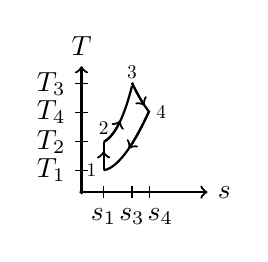
\begin{tikzpicture}[scale=.4,baseline={(0,0)}]
%\begin{tikzpicture}[show background rectangle, scale=.5]

%\draw (0,0) grid (4,4);
% x-axis
\draw [thick,->] (0,0) -- (4,0) node[right]{$s$};
% y-axis
\draw [thick,->] (0,0) -- (0,4) node[above]{$T$};
% x-axis label
%\node at (-0.3,4){$T$};
% y-axis label
%\node at (4,-0.3){$s$};
%origin point
\draw [color=black,fill=black] (0,0) circle (0.05);
%Isentropisk kompression
%x1=1.2, y1=1.958 till x2=1.2, y2=3.6
\draw[thick] (0.7,0.7)--(0.7,1.6) node[scale=0.7, above]{2};
\draw[thick,->] (0.7,0.7)--(0.7,1.3);

\draw (0.2,0.7)--(-0.2,0.7) node[left]{$T_1$};
\draw (0.7,0.2)--(0.7,-0.2) node[below]{$s_1$};

\draw (0.2,1.6)--(-0.2,1.6) node[left]{$T_2$};


%Isokor uppvärmning
%Isokor uppvärmning
%\node[scale=0.7,left] at (1,0.83){1};
\draw[ ->,rotate=7,thick,domain=0.9:1.5, smooth, variable=\x, black] plot ({\x}, {(1.46 + (\x-0.7)^2});
\draw[ rotate=7,thick,domain=0.9:2, smooth, variable=\x, black] plot ({\x}, {(1.46 + (\x-0.7)^2}) node[scale=0.7,above]{3};

\draw (0.2,{(2.8 + (1.5-0.7)^2})--(-0.2,{(2.8 + (1.5-0.7)^2}) node[left]{$T_3$};
\draw (1.6,0.2)--(1.6,-0.2) node[below]{$s_3$};

%Polytrop expansion n<kappa
%\node[scale=0.7, right] at (2,3.5);
%y= y0+(y1-y2)*abs((\x-x2)/(x2-x1))^n (2,3.15) -> (3.5,1.5)
%\draw[ thick,domain=1.2:1.9, smooth, variable=\x, black] plot ({\x}, {y0+(y1-y2)*abs((\x-x2)/(x2-x1))^n});
%\draw[ thick,domain=1.7:2.5, smooth, variable=\x, black] plot ({\x}, {1.5+(3.15-1.5)*abs((\x-3.5)/(3.5-2))^2});
\draw[ thick,domain=1.6:2.15, smooth, variable=\x, black] plot ({\x}, {(2+(3.5-0.5)*(abs((\x-3)/(1-3)))^2}) node[scale=0.7, right]{4};
\draw[ thick,->,domain=1.6:2, smooth, variable=\x, black] plot ({\x}, {(2+(3.5-0.5)*(abs((\x-3)/(1-3)))^2});
%\draw[ thick,->,domain=3:1.6, smooth, variable=\x, black] plot ({\x}, {(0.5+(3.5-0.5)*(abs((\x-3)/(1-3)))^2})

\draw (0.2,{(2+(3.5-0.5)*(abs((2.15-3)/(1-3)))^2})--(-0.2,{(2+(3.5-0.5)*(abs((2.15-3)/(1-3)))^2}) node[left]{$T_4$};
\draw (2.15,0.2)--(2.15,-0.2);
\node (A) at (2.5,-0.2)[below]{$s_4$};

%Isokor nedkylning
%\node[scale=0.7,left] at (1,0.83){1};
\draw[ ->,rotate=0,thick,domain=2.15:1.5, smooth, variable=\x, black] plot ({\x}, {(0.7 + (\x-0.7)^1.7});
\draw[ rotate=0,thick,domain=2.15:0.7, smooth, variable=\x, black] plot ({\x}, {(0.7 + (\x-0.7)^1.7}) node[scale=0.7, left]{1};



%Pilar
%\usetikzlibrary {arrows.meta}
%\draw [arrows ={-Stealth[scale=1]}] (1.5,2.5) -- (1.5,1.9);
%\draw [arrows ={-Stealth[scale=1]}] (1.75,1.5) -- (1.75,1.0);
%\path (1.2,2.8) node  {$q_{till}$};
%\path (1.6,0.4) node  {$q_{\textit{bort}}$}; 

\end{tikzpicture}
}
%    \caption{Mät 2}
\label{fig4}
%\caption{Anpassning av $n$ i $p=\frac{C}{V^n}$}
\end{figure}

Den teoretiska termiska verkningsgraden $ \eta_t $ definieras enligt
%\begin{wrapfigure}[5]{l}{0cm}
\begin{flalign*}
\eta_t &=\frac{q_{tillf}-|q_{bortf}|}{q_{tillf}} &\\
       &=1-\frac{|q_{bortf}|}{q_{tillf}} & (1)\\
\end{flalign*}

$q_{tillf}$ består av den värmeenergi som tillförs under isokor uppvärmning
$q_{23}$ samt värmetillförseln under isotropiska expansionen $q_{34}$ eftersom
integralen från $2$ till $4$ i $T\mhyphen s$-diagrammet är positiv då processpilen
löper i positiv riktning, $ds>0$. Definitionen för entropi är
\begin{flalign*}
ds &= \bigg( \frac{dq}{T}\bigg)_{rev} &(2)\\    
\end{flalign*} 
Att $q$ är arean under kurvan i $T\mhyphen s$-diagrammet som kan ha olika
tecken beroende på om integration sker till höger eller vänster
förstås från följande likheter som följer ur definitionen för entropi.
\begin{flalign*}
\int T\cdot ds &= \int dq  &\\
\int T\cdot ds &=q   &(3)\\
\end{flalign*}
För fullständighetens skull anges också entropidefinitionen för en icke-reversibel process.
\begin{flalign*}
ds &=  \frac{dq}{T} + \frac{|dw_f|}{T}&(4)\\    
\end{flalign*}
där $dw_f$ är friktionsarbetet uttrycket per massenhet.
Entropin blir alltså större med friktionsvärme eftersom friktionstermen
adderar till högerledet av uttrycket för en reversibel process.

Den bortförda värmeenergin $q_{bortf}$ sker under den isokor-processen från $4$
till $1$, $q_{bortf} = q_{41}$.

Vi börjar med att teckna $q_{tillf}$ som är $q_{23}$ + $q_{34}$.
$q_{23}$ är värmen som tillförs under en isokor.
\begin{flalign*}
dq_{23} &= du + p\cdot dv &\\
        &= du + p\cdot 0 &\\
q_{23} &=\int_2^3 du &\\
       &=\int_2^3\bar{c}_v\cdot dT &\\
        &=\bar{c}_v\cdot(T_3-T_2) &(5)\\
\end{flalign*}
Har vi värden på $\bar{c}_v$, $T_3$ och $T_2$?\hfill\break
Information om $T_3$ har vi men $T_2$ och $\bar{c}_v$ är okända
\begin{flalign*}
q_{23} &=\mycirc{$\bar{c}_v$}\cdot(T_3-\mycirc{$T_2$}) &\\
\end{flalign*}
Vi vet endast att det rör sig om en ideal gas.
Med de siffervärden som vi känner till så har vi i alla fall
\begin{flalign*}
q_{23} &=\bar{c}_v\cdot(700-T_2) &(6)\\
\end{flalign*}


För att teckna  $q_{34}$ som är den andra termen i summan för $q_{tillf}$  så måste vi härleda
ett uttryck för $dq$ specifikt för en polytrop process.
Från termodynamikens första huvudsats har vi $dq = du + p\cdot dv$, vilket kräver att vi måste
teckna ett uttryck för volymändringsarbetet $p\cdot dv$
För polytropiska processer gäller
\begin{flalign*}
p_1\cdot V_1^n &= p_2\cdot V_2^n &  \\
p\cdot V^n &=\  \text{konstant} & (7)\\
\end{flalign*}
Tar vi naturliga logaritmen på båda sidor av (7) så får vi
\begin{flalign*}
ln\ p + n\cdot ln\ V &=\ \text{konstant} & (8)\\
\end{flalign*}
Detta är lösningen till differentialekvationen
\begin{flalign*}
\frac{dp}{p}+n\cdot\frac{dV}{V}&=0 & (9)\\
\end{flalign*}
Vi multiplicerat vänster- och höger-led med $p\cdot V$ och får
\begin{flalign*}
V\cdot dp + n\cdot p\cdot dV &= 0 &(10)\\
\end{flalign*}

Om vi tar ln-funktionen på allmänna gaslagen så får vi
\begin{flalign*}
ln\ p + n\cdot ln\ V &= m\cdot R+ ln\ T & (11)\\
\end{flalign*}
Vilket är en av många lösningar till differentialekvationen
\begin{flalign*}
\frac{dp}{p}+\frac{dV}{V}&=\frac{dT}{T} & (12) \\
\end{flalign*}
Multiplicerar vi (12) med $p\cdot V$ så får vi
\begin{flalign*}
V\cdot dp + p\cdot dV &= p\cdot V \frac{dT}{T} &(13)\\
\end{flalign*}
Men denna kan skrivas med allmänna gaslagen på formen
\begin{flalign*}
\frac{p\cdot V}{T}&= m\cdot R
\end{flalign*}
\begin{flalign*}
V\cdot dp + p\cdot dV &= m\cdot R\cdot dT & (14)\\
\end{flalign*}
Subtraheras (14) från (10) fås
\begin{flalign*}
V\cdot dp + n\cdot p\cdot dV &-V\cdot dp + p\cdot dV &\\
                             &=0-m\cdot R\cdot dT &\\
(n-1)\cdot p\cdot dV &= -m\cdot R\cdot dT & \\
\end{flalign*}
Vi kan lösa ut $p\cdot dV$ och får
\begin{flalign*}
p\cdot dV &=-\frac{m\cdot R\cdot dT}{n-1}  &(15)\\
\end{flalign*}
Uttryckt per massenhet $(v=V/m)$ så fås
\begin{flalign*}
p\cdot dv &=-\frac{R\cdot dT}{n-1}  &(16a)\\
\end{flalign*}
Denna kan vi också skriva om med $\bar{c}_v$ och $\kappa$ eftersom
$R= \bar{c}_v\cdot (\kappa -1)$
\begin{flalign*}
p\cdot dv &=-\frac{\bar{c}_v\cdot (\kappa -1)}{n-1}\cdot dT  &(16ab)\\
\end{flalign*}

Vi kan nu beräkna värmemängdsändringen per massenhet $q$ för en polytrop process
\begin{flalign*}
dq &= du + p\cdot dv &\\
   &= \bar{c}_v\cdot dT -\frac{R\cdot dT}{n-1} &\\
   &= \bar{c}_v\cdot dT -\frac{\bar{c}_v\cdot (\kappa -1)}{n-1}\cdot dT &\\
   &= \bar{c}_v\bigg(\frac{n-1}{n-1} -\frac{ \kappa -1}{n-1}\bigg)\cdot dT &\\
    &= \bar{c}_v\cdot \frac{n-\kappa}{n-1}\cdot dT &\\
\end{flalign*}
Integreras denna från 3 till 4 så fås
\begin{flalign*}
q_{34} &=\int_3^4\bar{c}_v\cdot \frac{n-\kappa}{n-1}\cdot dT &\\
       &=\bar{c}_v\cdot\frac{(n-\kappa )}{n-1}\cdot (T_4-T_3)&(17)\\
\end{flalign*}
med insättning av det som vi har information om så fås
\begin{flalign*}
q_{34} &= \bar{c}_v\cdot (500-700)\cdot\frac{1.2-1.4 }{1.2-1}&\\
       &=\bar{c}_v\cdot 200 &(18)\\
\end{flalign*}
Vi har nu sammanfattningsvis $q_{tillf}$ enligt
\begin{flalign*}
q_{tillf} &= q_{23} + q_{34} &\\
          &= \bar{c}_v\cdot(700-T_2)+\bar{c}_v\cdot 200 &(19)\\
\end{flalign*}
$q_{bortf}$ är endast den isokora nedkylningen från $(4)$ till $(1)$ 
$q_{bortf}=q_{41}$ således
\begin{flalign*}
q_{41} &= \bar{c}_v\cdot (T_1-T_4) &\\
       &= \bar{c}_v\cdot (300-500) &\\
q_{bortf}&=-\bar{c}_v\cdot 200 &(20)\\
\end{flalign*}
Men vi är faktiskt endast intresserade av $|q_{bortf}|$
\begin{flalign*}
|q_{bortf}| &= \bar{c}_v\cdot 200 &(21)\\
\end{flalign*}
Vi saknar information om $T_2$. Att vi inte har något värde på $\bar{c}_v$ spelar ingen
roll därför att vi kommer att kunna förkortas bort denna
när kvoten $|q_{bortf}|/q_{tillf}$ tecknas.

Tipset i boken är att inse att 
\begin{flalign*}
s_4-s_1 &= (s_4-s_3) + (s_3-s_2) &(22)\\
\end{flalign*}
Vi behöver uttrycken för entropiändringarna för isokor-processerna dvs. för $(s_4-s_1)$ och $(s_3-s_2)$
samt för polytrop-processen $(s_4-s_3)$.
Dessa kan vi ta direkt ur formelsamligen men vi väljer här att genomföra dessa
beräkningar. Nu har ju vi data för en processen som går från (4) till (1) och bör kanske beräkna
$s1-s4$ men detta är ju inget annat än -$(s_4-s_1)$, så vi räknar som om processen gick från $(1)$ till $(4)$
För isokorprocesser gäller som bekant att $dv=0$ där för blir $ds$ på följande vis
\begin{flalign*}
ds &= \bigg( \frac{dq}{T}\bigg)_{rev} &\\ 
   &=\frac{du}{T} + \frac{p\cdot dv}{T} &\\
   &=\frac{\bar{c}_v\cdot dT}{T}&\\
\end{flalign*}
Integrering ger
\begin{flalign*}
\int_1^4 ds &= \int_1^4 \frac{\bar{c}_v\cdot dT}{T} &\\
s_4 - s_1 &=  \bar{c}_v\cdot ln\bigg(\frac{T_4}{T_1}\bigg) &(23)\\
\end{flalign*}
Likaså kan vi beräkna $s_3-s_2$ för isokoren från $2$ till $3$
\begin{flalign*}
s_3 - s_2 &=  \bar{c}_v\cdot ln\bigg(\frac{T_3}{T_2}\bigg) &(24)\\
\end{flalign*}
För den polytropa processen $3$ till $4$ så har vi
\begin{flalign*}
ds &= \bigg( \frac{dq}{T}\bigg)_{rev} &\\ 
   &=\bar{c}_v\cdot \frac{n-\kappa}{n-1}\cdot\frac{ dT}{T} &\\
\end{flalign*}
Integreras $ds$ från 3 till 4 så fås
\begin{flalign*}
\int_3^4 ds &= \int_3^4 \bar{c}_v\cdot \frac{n-\kappa}{n-1}\cdot\frac{ dT}{T} &\\
s_4 - s_3 &=  \bar{c}_v\cdot \frac{n-\kappa}{n-1}\cdot ln\bigg(\frac{T_4}{T_3}\bigg) &(25)\\
\end{flalign*}
Vi tecknar nu uttrycken för $(s_4-s_1)$=\hfil\break $(s_4-s_3)+(s_3-s_2)$ och ser om vi kan lösa ut $T_2$
\begin{flalign*}
s_4-s_1 &= (s_4-s_3) + (s_3-s_2) &\\
\bar{c}_v\cdot ln\bigg(\frac{T_4}{T_1}\bigg) &= \bar{c}_v\frac{n-\kappa}{n-1}\cdot ln\bigg(\frac{T_4}{T_3}\bigg) &\\
                                             &\ +\bar{c}_v\cdot ln\bigg(\frac{T_3}{T_2}\bigg) &\\
\end{flalign*}
Vi kan börja med att förkorta bort $\bar{c}_v$
\begin{flalign*}
ln\bigg(\frac{T_4}{T_1}\bigg) &= \frac{n-\kappa}{n-1}\cdot ln\bigg(\frac{T_4}{T_3}\bigg) &\\
                              &\ +ln\bigg(\frac{T_3}{T_2}\bigg) &\\
\end{flalign*}
Vi kan förbereda vänster- och höger-led för att ta ta e-upphöjt av vänster och höger-led
\begin{flalign*}
ln\bigg(\frac{T_4}{T_1}\bigg) &= ln\Bigg[\bigg(\frac{T_4}{T_3}\bigg)^{\frac{n-\kappa}{n-1}}\Bigg] &\\
                              &\ +ln\bigg(\frac{T_3}{T_2}\bigg) &\\
\end{flalign*}
Nu tar vi e-upphöjt.
\begin{flalign*}
\frac{T_4}{T_1} &= \bigg(\frac{T_4}{T_3}\bigg)^{\frac{n-\kappa}{n-1}}\cdot \frac{T_3}{T_2} &(26)\\
\end{flalign*}
Högerledet måste bli en produkt därför att potenslagarna säger att $e^{\alpha + \beta}$ = $e^\alpha\cdot e^\beta$.
Om $\alpha$ och $\beta$ är ln-funktioner så blir resultatet produkten av argumenten för
ln-funktionerna.
\begin{flalign*}
T_2 &= \bigg(\frac{T_4}{T_3}\bigg)^{\frac{n-\kappa}{n-1}}\cdot \frac{T_3\cdot T_1}{T_4} &\\
    &= \bigg(\frac{500}{700}\bigg)^{\frac{1.2-1.4}{1.2-1}}\cdot \frac{700\cdot 300}{500}&\\
    &=588^{\text{o}}\text{K}&(27)\\
\end{flalign*}

Nu är det bara sätt in i formeln för verkningsgraden. 
\begin{flalign*}
\eta_t &=1-\frac{|q_{bortf}|}{q_{tillf}} &\\
       &=1-\frac{\bar{c}_v\cdot 200}{\bar{c}_v\cdot(700-588)+ \bar{c}_v\cdot 200}&\\
       &=1-\frac{200}{312}&\\
       &=1-0.641025641&\\
       &=0.358974359
\end{flalign*}
Svar med korrekt antal värdesiffror måste vara med två värdesiffror eftersom det minsta antalet värdesiffror
av en parameter i problemformuleringen var för $\kappa=1.4$
Således skall svaret vara $\eta_t=0.36$ eller 36\%

%\end{multicols}
%\listoffigures
%\listoftables
%\tableofcontents

\end{document}
